%%%%%%%%%%%%%%%%%%%%%%%%%%%%%%%%%%%%%%%%%%%%%%%%%%%%%%%%%%%%%%%%%%%%%%%%%%%%%%%%%%%%%%%%%%%%%%%%%%%%%%%%%%%%%%%%%%%%%%%%%%%%%%%%%%%%%%%%
% This is just a template to use when submitting manuscripts to Frontiers, it is not mandatory to use frontiers.cls nor frontiers.tex  %
%%%%%%%%%%%%%%%%%%%%%%%%%%%%%%%%%%%%%%%%%%%%%%%%%%%%%%%%%%%%%%%%%%%%%%%%%%%%%%%%%%%%%%%%%%%%%%%%%%%%%%%%%%%%%%%%%%%%%%%%%%%%%%%%%%%%%%%%

\documentclass{frontiersENG} % for Engineering articles
%\documentclass{frontiersSCNS} % for Science articles
%\documentclass{frontiersMED} % for Medicine articles

\usepackage{url,lineno}
\linenumbers

\usepackage{graphicx}

% Leave a blank line between paragraphs in stead of using \\

\copyrightyear{}
\pubyear{}

\def\journal{Neuroinformatics}%%% write here for which journal %%%
\def\DOI{}
\def\articleType{Research Article}
\def\keyFont{\fontsize{8}{11}\helveticabold }
\def\firstAuthorLast{McCormick {et~al.}} %use et al only if is more than 1 author
\def\Authors{Matthew McCormick\,$^{1,*}$,
  Xiaoxiao Liu\,$^{1}$,
  Julien Jomier\,$^{2}$,
  Charles Marion\,$^{2}$,
  and Luis Ibanez\,$^1$}
% Affiliations should be keyed to the author's name with superscript numbers and be listed as follows: Laboratory, Institute, Department, Organization, City, State abbreviation (USA, Canada, Australia), and Country (without detailed address information such as city zip codes or street names).
% If one of the authors has a change of address, list the new address below the correspondence details using a superscript symbol and use the same symbol to indicate the author in the author list.
\def\Address{$^{1}$Medical Computing Group, Kitware Inc, Clifton Park, NY, USA\\
$^{2}$Medical Computing Group, Kitware Inc, Lyon, France\\
$^{3}$University of Michigan, Ann Arbor, MI, USA\\
}
% The Corresponding Author should be marked with an asterisk
% Provide the exact contact address (this time including street name and city zip code) and email of the corresponding author
\def\corrAuthor{Matthew McCormick}
\def\corrAddress{Medical Computing Group, Kitware Inc, Clifton Park, NY, USA}
\def\corrEmail{matt.mccormick@kitware.com}

% \color{FrontiersColor} Is the color used in the Journal name, in the title, and the names of the sections


\begin{document}
\onecolumn
\firstpage{1}

\title[ITK Reproducible Research]{ITK: Enabling Reproducible Research and Open Science}
\author[\firstAuthorLast ]{\Authors}
\address{}
\correspondance{}
\extraAuth{}% If there are more than 1 additional author, comment this line and uncomment the next one
%\extraAuth{corresponding Author2 \\ Laboratory X2, Institute X2, Department X2, Organization X2, Street X2, City X2 , State XX2 (only USA, Canada and Australia), Zip Code2, X2 Country X2, email2@uni2.edu}
\topic{Research Topic}

\maketitle
\begin{abstract}

Reproducibility verification is essential to the practice of the scientific
method. As researchers report their findings to the public, what enables such
findings to be considered part of the knowledge base of the scientific
community is whether they have been replicated by independent groups or not. In
the many scientific fields where software has become a fundamental tool for
capturing, and analyzing data, this requirement of reproduciblity implies that
reliable and comprehensive software platforms and tools should be made
available to the scientific community, to empower them and the public, to verify
in practice the reproducibility of observations that are reported in the
scientific literature.

Medical image analisys is one of the fields in which the use of computational
resources, both software and hardware, are an essential platform for performing
experimental work. In this arena, the introduction of the Insight Toolkit (ITK)
in 1999 has transformed the field, and propulsed its progress by accelerating
the rate at which algorithmic implementations are developed, tested,
disseminated and improved. By building on the efficiency and quality of Open
Source methodologies, ITK has provided the medical image community with an
effective platform on which to build a daily workflow that incorporates the
true scientific practices of reproducibility verifcation.

This article describes the multiple tools, methodologies and practices that the
ITK community has adopted, refined and followed during the past decade, in
order to become on of the research fields with the most modern reproducibility
verification infrastructure. Some of the elements described here include
software development methodologies, advanced publishing practices, and a
cohesive community culture.

\section{}
%As a primary goal, the abstract should render the general significance and
%conceptual advance of the work clearly accessible to a broad readership.
%References should not be cited in the abstract.

%See the Summary Table at \\
%\url{http://www.frontiersin.org/}\texttt{\journal}\url{/authorguidelines}
%\\for abstract requirement and length according to article type.

\tiny
 \keyFont{ \section{Keywords:} Reproducibilty, ITK,Insight Journal, Code Review, Open Science} %All article types: you may provide up to 8 keywords; at least 5 are mandatory.
\end{abstract}


\section{Introduction}

% For Original Research Articles, Clinical Trial Articles, and Technology
% Reports the introduction should be succinct, with no subheadings.
%
%For Clinical Case Studies the Introduction should include symptoms at
%presentation, physical exams and lab results.
%
The essential feature of the scientific method is the practice of verification
of reproducibility.The large majority of research activity today is focused on
generating novelty, and only in exceptional cases, concerned with the
verification of reproducibility. The practice of peer-review has been assumed
to be a suitable replacement for the verification of reproducibility, a mistake
by which experimental work has been replaced by thought experiments and
opinion-based evaluations that do little to further the scientific enterprise.
This drift has denigrated, what used to be scientific work, back into the
practice of the ``natural philosophy'' in which we simply imagine models of the
natural word and evaluate them based on aesthetic appeals and desire for
self-consistency.

The Insight Toolkit (ITK) has made it possible to restore the true practice of
the scientific method in the field of medical image analysis. By providing a
common platform in which image analysis algorithms and processing techniques
can be implemented and can be freely disseminated. ITK empowers all to verify
the experimental work of image analysis research activities. This of course,
requires that researchers adhere to the true practice of the scientific method
and publish the full details of their methodology, including the source code,
data, parameters and auxiliary documents that are required for a third party to
independently repeat the work and verify the findings.

The ITK community created in 2005 a scientific journal, the Insight Journal,
truly fulfilling the practice of the scientific method, where all articles are
required to provide the full set of source code, data and parameters needed to
reproduce the finding of the authors. These materials are immediately made
available to readers and reviewers, empowering them to indeed perform such
verification with minimal effort and minimal loss of information.

Other Journals, in particular Frontiers, PLoS, and more recently Nature, have
embraced this restoration of the true practice of the scientific
method~\cite{NatureEditorial2013,NatureEditorial2012,Mobley2013}.  With the
support of the Reproducible Research movement, these progressive publication
venues are creating the conditions for a new age of enlightenment in which the
methodologies of practical research work will not be subject to secrecy, nor be
subject to the veil of suspicion that many incidents of scientific fraud and
data manufacturing that have left us with in recent months~\cite{Sandve2013}.


The National Library of Medicine’s Insight Segmentation and Registration
Toolkit (ITK) was conceived in 1999 to support analysis of The Visible Human
Project data. In order to maximize its impact, the project embraced an open
source development model from its inception. Not only was the project
successful in its original objective, it also extended far beyond its original
goals and became a foundational component of many National Institutes of Health
(NIH) research projects, as well as evolved into a technology underlying many
medical image analysis commercial products worldwide.

%
%The following numbers were computed with the script:
%src/git-lines-of-code-statistics.sh
%
The ITK repository currently contains over 2.5 million lines of source code
(including 1.2 million lines of third-party code added to the repository).
Contributions to this repository can be measured by the number of logical
changes made to the code, also known as commits, and the number of source code
line additions or deletions. In its 14 years of history, ITK has received
37,626 commits, in 13,184 files, by 209 different authors.

Ohloh.net \cite{OhlohITK2013} is a public directory of open source projects
that performs analytics on the code history of communities surrounding
projects. According to its Project Cost Calculator, the effort in the toolkit
is an estimated 730 person-years, amounting to an estimated cost of 40 million
dollars given an average salary of \$55,000 per year.

As of October 29, 2013, the combined subscribers to the \textit{community},
\textit{insight-users}, and \textit{insight-developers} mailing lists are 2,698.
The lists average 326 messages per month from October 2012 to October 2013.


\section{Materials \& Methods}

\subsection{Reproducibility Assurance Practices}

The practice of reproducibility verification requires that the software
platforms and tools used to support research activities be built in an
environment that ensures their high quality, consistency and reliability. This
leads to a continuous interplay between correctness and consistency. More
explicitly, it would be ideal to expect that running an experiment multiple times
would yield consistently the same results. It is ideal if this holds as more
recent versions of software tools are used to support the given experiment.
However, at the same time, software goes through a continuous process of
improvement, modification and correction. Therefore, changes are flowing on a
steady manner into the code base. To balance the benefits and challenges of
this interplay, it is essential to use both a set of software quality support
tools, and a set of community practices that make proper use of such tools.

To ensure the code quality of the toolkit and the growth of the ITK community,
adaptation to modern software practices are necessary. In particular, the
recent modernization of ITK includes adopting a version control system (Git),
 a code review system (Gerrit), a Gerrit-integrated dashboard testing system
(CDash@Home), and modularization of the toolkit.

\subsubsection{Source Code Version Control: Git} Version control is an
essential practice that must be applied to all software used to support the
quest for knowledge in a reproducible research environment. A good source code
version control system allows developers to easily keep track of the entire
history of the software development. Git is an open source, distributed version
control system designed to perform with speed and efficiency. Its features
include easy local branching, convenient staging areas, and multiple workflows,
which are particularly useful for large open source projects like ITK.

The ITK community embraced the used of Git as part of the modernization activites
leading to ITKv4 in 2010.  When migrating the source code repository from CVS
to Git, the history of the development was preserved and a simple Git workflow
was customized for ITK developers.  The adoption of Git empowered ITK
developers to easily create flexible workflows of branching and merging. It
also allowed developers to make commits in local repositories, and hence
enabled them to work consistently even when not connected to the network.

Despite the initial step learning curve to learn commonly used Git commands,
Git provides a superior, welcoming collaboration platform for the community. It
has become the new standard for source code version control.  And more
importantly, great tools that are base on Git are accessible to ITK, such as
the peer code review system: Gerrit Review.

\subsubsection{Open Review System: Gerrit Review} In the context of
reproducible science, the detailed description of the methods and materials
used to perform an experiment are a fundamental piece of the article that
disseminates the results. As research activities become more and more dependent
on software for the preparation, execution and analysis of experiments, it
becomes necessary to include all the details related to the software as part of
a reproducible publication. Given the complexities of software implementation,
mere algorithmic descriptions, or even pseudo-code, are not sufficient to ensure
reproducibility through reimplementation. Only the delivery of original source
code can provide enough assurances that the recipient of the materials will be
able to replicate the reported work with a reasonably limited amount of effort.

The code must therefore be subject to peer review processes similar to the ones
currently used for scientific publications. Such reviews should examine both
the quality and correctness of the code, as well as proceed to verify the
reproducibility of the code through its actual execution.

Recently, recognition of software's importance for the progress of science has
elicited movements such as the ``Science Code Manifesto''~\cite{Barnes2011}.
While a number of journals are beginning to adopt practices similar to The
Insight Journal, where code is submitted along with the article, evaluation
tools and procedures for peer review of the code are not in parity with those
used for the article. Commonplace practices have evolved to facilitate article
review such as evaluation rubrics, instrumentation of the text with line and
page numbers for reference during discussion, and a process to distribute an
article to reviewers and communicate author replies.  While this provides the
reviewers with a mechanism to evaluate the reproducibility, and therefore the
merit, of the article, the technical nature of code solicits greater technical
capabilities of the tools and methods used to evaluate its reproducibility.

While this problem is multi-faceted, some progress has been made through ITK’s
adoption of the Gerrit Code Review system.  Gerrit is an open source project
maintained by the Google Android mobile phone project. This systems enables a
large community of developers to inspect and comment on the code changes that
are proposed for inclusion in a software system. Not only has the ITK community
embraced the use of Gerrit, it has also contributed fixes and features back to
the upstream Gerrit project.

Gerrit is implemented as a combination of a web-based front end with a Git
repository backend. Most of the interactions that developers have with Gerrit,
happen with the web-based front end server. The Gerrit server provides a
mechanism to effectively evaluate code changes, obtain and test those changes
locally, and perform notification and transmission of the changes and comments
for authors and reviewers, as well as management of the system to accept
merges.

Gerrit is a technology that is built around the Git distributed version control
system.  With Git, contributors can independently develop and test patches that
are put in topic branches created out of the ITK master branch.  Next, the
patch can be shared with the community by pushing the topic branch to the
Gerrit server \cite{ITKGerrit}.  Once in the server, the change is publicly
accessible via the web-based front end.  Developers can then use a web-browser
to see side-by-side differences that are easily identified with
color-highlighting, on a file-based diff page.

From the web interface, contributors can request the attention of specific
reviewers to comment on their patch. As a convenience, the web-interface
provides auto-completion of names for any community member that has registered
an account with the server.  The reviewers for a given change can be added or
removed throughout the review process by any community members, and they will
be notified via email of any new comments or change revisions.  In the Gerrit
system, every change is identified by a unique Change Id, which allows multiple
revisions, also known as Patch Sets, to be uploaded consistently in response to
comments.

The discussion of the change between author and reviewers occurs via three
mechanisms: overall comments on the change, inline comments, and numerical
ratings. Overall comments conveying general remarks can be added per Patch
Set, and the history of comments is retained and easily navigated. Questions
and suggestions can be directed at specific sections of the code with the
inline comments. Whether the code can reproducibly be built and pass tests is
indicated by the reviewer with a numerical Verified score, and overall
evaluation is indicated with a numerical Code Review score. With the Gerrit
Code Review system, reproducibility is improved through continual refinement of
the corpus of Insight Toolkit knowledge, as embodied in the code repository,
through experimentation as implemented in the unit tests and through peer
review as exercised in the code reviews.

\subsubsection{Open Dashboard} ITK has a stringent system of quality control
that uses a combination of unit testing, regression testing, multi-platform
verification, and continuous integration. The testing infrastructure of ITK
includes more than 2,400 unit tests, which provide a code coverage of 84\% of
ITK code lines.

The collection of unit tests are executed nightly by computers contributed by
community members all around the world, and reporting to a central online
dashboard that summarizes the results. This web-based dashboard system (CDash)
 \cite{ITKDashboard} ensures ITK$'$s software quality as developers around the
world continuously make changes to the code base. Build status and regression
test status are visualized in a tabular form. The dashboard is an important
coordination and communication tool that empowers developers to share the
results of a local test with other developers by pushing them to the online
summary pages.

Continuous builds triggered by patches submitted to the Gerrit code review
system also give feedback to developers on the impact of recent changes.
Nightly builds of the project spanning a wide variety of platforms and
configurations ensure that ITK can be built on a diversity of operating systems
and hardware.



\subsection{Sustainability}

In order to facilitate the long term viability of a project, it is essential to
cultivate an active community around it. The adoption of proper cultural
practices by the community ensure the long term quality and sustainability of
the project, in a manner that is consistent with the principles of
reproducibility and therefore, with the practices of open science.

\subsubsection{Community Enablement}

The ITK community has cultivated a number of practices intended to ensure that
the demographics of contributors are continously renewed. In this way, the
community remains active and vibrant, and can provide the manpower needed to
maintain and improve the Insight Toolkit. In particular, this involves welcoming
new members and training them on:  technical skills, social rules, governance
processes, and cultural practices.

On the training front, the ITK community has been hosting a series of webinars
to promote ITK in general and the new features available in ITK version 4
(ITKv4) in particular. The webinar videos have been posted publicly, and have
received more than 1,000 plays so far. As the number of webinars grow, they
also start covering more advanced topics, such as the porting of ITK to
devices based on the ARM architecture, with webinars such as ``Raspberry Pi
Likes ITK'' and ``Raspberry Pi Likes ITK with VTK'', that describe how to use
ITK in the highly popular Raspberry Pi board.

To empower new developers and lower the barrier of entry for new users, a web
site was put in place to host and distribute a large collection of examples on
various ITK classes and filters (\url{http://itk.org/ITKExamples}).

In a very focused effort to grow the ITK community, an online space called
ITKBarCamp (\url{http://insightsoftwareconsortium.github.io/ITKBarCamp-doc/})
was created to train new community members on the software technologies that
are essential to ITK. This space provides a combination of training materials,
such as source code, documentation and video tutorials, that guide newcomers at
their own pace through training activities aimed at honing their software
development skills.

One of the very active areas in the ITK BarCamp is a series of participatory,
short YouTube.com videos with associated documentation covering various topics
related to ITK, including:

\begin{enumerate}
\item Mastery of the command line
\item Basic C++ programming skills
\item Good software practices, including unit testing
\item Recommended tools and workflows for ITK development.
\end{enumerate}

So far 29 short tutorial videos have been created, which have received 2,234
views and attracted 30 subscribers. ITK Bar Camp materials are hosted in Github
as written documentation with references to video archives. Information on
previous and current webinars and hangouts can be found at
(\url{http://www.itk.org/ITK/resources/webinars.html}).

These educational efforts are crucial to attracting, training, and retaining
new community members in the long run, and through that mechanism replenish the
community with active members. We plan to continue creating ITK Bar Camp
tutorials and to encourage other community members to contribute to the
repository.

\subsubsection{Modularization}
Since its inception in 2000, ITK was designed as a collection of about seven
core libraries and about ten third party libraries.  This monolithic
organization of the code led over time to very large sub-libraries, as more
classes were added to the toolkit. Once the core code of ITK surpassed
half-a-million lines of code, it became evident that a more modular approach
was needed in order to support the future continued growth of the toolkit.

\textbf{Figure 1.}{An illustration of ITK modules' dependencies.}\label{fig:01}

Such modularization was implemented in 2010-2011 as part of the larger
refactoring effort leading to ITKv4.  As a result of the modularization, the
initial monolithic code base of about 12,000 files was partitioned into more
than 100 modules.  And as of Oct of 2013, ITK main code repository contains
137 modules in total.

Dependencies, Figure \ref{fig:01}), between modules were identified and
explicitly declared in the CMake-based \cite{CMake} configuration system. By making the
CMake-based configuration system aware of the new ITK modularization, ITK
adopters became enabled to select, at configuration time, the pieces of ITK
that they wanted to use in their own projects.

Support for adding Remote Modules was also built into the ITK modularization
infrastructure. These are modules that can be coupled with a particular
ITK source code installation, without the requirement to be incorporated directly into
the official ITK repository. By making it possible for adopters to integrate
new modules, the Remote Module infrastructure enables fast
dissemination of research code through ITK without increasing the size of the
main repository. These Remote Modules can be exchanged across members of the
community based upon interest and need, which accelerates the rate
of dissemination of emerging modules as well as helping those modules mature
faster through the rapid use, testing, and commentary by early adopters. Currently
there are four ITK remote modules hosted on GitHub.

\textbf{Figure 2.}{ Code contribution process in ITK.}\label{fig:02}

The modularization effort significantly improves the extensibility of the
toolkit and lowered the barrier of contribution. A recommended contribution
process is illustrated in Figure \ref{fig:02}.  All new modules can be dropped
into the ITK source tree as external modules for testing, and they should be
submitted to Insight Journal for review. Once the External module passes
dashboard testing and peer review, it can be submitted as a Remote module. As
a result, it will be disseminated from ITK itself while its source code is
maintained independent of the main ITK repository. Specifically, the source
code of a Remote module can be downloaded via CMake at CMake configuration
time, which makes it a convenient method to distribute modular source code
without increasing the size of the main repository. After the Remote Module
has experienced sufficient testing and community members express broad
interests in the contribution, the submitter can then move the contribution
into the ITK repository via Gerrit code review.  It is possible but not
recommended to directly submit a module to Gerrit for review without
submitting to Insight Journal first. An Insight Journal article describing the
background, functionalities, and the design behind the module is a great way
to provide extra documentation.


\subsection{Open Publication: The Insight Journal}
ITK was conceived as a usable encyclopedia of image analysis algorithms
that are of particular utility to the medical imaging community. Given the
rapid pace at which technology develops in this area, and the proliferation of
both generic and specialized image analysis algorithms, it is important for ITK
and its community to continuously update the content of the toolkit by adding
new algorithms while simultaneously improving and extending existing ones. To
do this, the ITK community relies on contributions made by its members as they
use the toolkit to support their own projects and run into situations where
additions and improvement are required for them to achieve their goals. In
order to absorb these contributions, the ITK community has used the Insight
Journal \cite{InsightJournal} since 2005. The online Insight Journal
publishes practical articles written by developers for developers and requires
those articles to be fully reproducible.

The Insight Journal is a free, open-access publication covering the domain of
medical image processing and visualization. It enables community members to
publish their contributions to medical projects for open peer-review, full
reproducibility verification, and open-rating by readers worldwide.

%
%  the following statistics were obtaines with the script
%
%            src/insight-journal-statistics.sh
%
The journal is very active, and since its inception in 2005, it has published
564 articles with 809 public reviews and has more than 2,600 subscribed
readers. Just the top five most popular articles have been downloaded more than
5,000 times each, for a combined number of 43,384 downloads and combined number
of 71,500 views. The Insight Journal is currently the only technical
publication in the domain of image analysis that not only allows but also
requires verification of reproducibility as part of the submission and review
process. The importance of restoring the practice of reproducibility
verification in scientific research has resurged in recent years in light of
worrisome findings of inconsistency, lack of quality and even fraud in what
were otherwise considered to be high-quality publications \cite{Begley2012}. By
adhering to a reproducibility verification requirement, the Insight Journal
ensures that community members get rapid access to reliable publications that
include open source software that they can readily use in their projects.

The Insight Journal now accepts ITK module submissions. This feature empowers
community members to take advantage of the new modular structure in ITK and
makes future code integration easier. Readers can then download Insight Journal
articles and directly plug them in as Remote Modules on their local ITK
installation.


\section{Results}

\subsection{Contribution Statistics}

\textbf{Figure 3. }{Histogram of ITK contributors by number of commits in the repository since 2000.}\label{fig:03}

Figure 3 shows the distribution of contributions
to the source code base of the ITK toolkit. Every bar corresponds to an individual
contributor. The height of the bar represents the number of commits that this
contributor has authored. The figure shows the top 100 contributors, out of a
total of 207. The ITK community follows a typical power-law distribution, where
a concentrated number of contributors are responsible for the majority of the
commits, while a large number of contributors make small contributions.  This
phenomenon is known as the ``Long Tail'', and it is quite important for the
structure of the community. The long tail of contributors who make small
changes are an important strength of the community since they tend to provide
the majority of the quality control after versions of the software have been
released. The head and the tail of the distribution have interacting dynamics
that complement each other and ensure that innovation makes its way into the
software, while at the same time it matures and gets adjusted to the true needs
of the larger number of adopters.

\subsection{Software Quality Assurance}

When integrating the contributions of a large number of community members, it
is vital to have in place a quality control mechanism. This
eliminate defects in the code before they are introduced into the repository, and
it also ensures consistency and coherency across the toolkit.
The quality assurance infrastructure of ITK is implemented by a combination
of several interacting tools. In particular: the configuration system CMake,
the online quality control dashboard CDash, the revision control system Git,
and the code review system Gerrit. This infrastructure is complemented by
coordination and communication tools such as mailing lists, wikis,
weekly phone calls, and regular online videoconference meetings.

The life cycle of a code change starts in the communication channels when
community members raise issues in the code. These issues might relate to lack
of correctness, or lack of desirable features, run-time performance
bottlenecks, lack of support for specific platforms, or
problems with specific types of data. Typically, the issues are discussed among
community members until it is determined that changes in the code are required,
and that one or several community members will take on the task of
implementing the required changes.

Once community members prepare initial versions of the required changes, they
commit them in their local clones of the Git repository, from where they can
submit them to the peer code review tool, Gerrit. A group of two or three reviewers
are invited to review and test the code contributions and a conversation
ensues, where the submitters and reviewers iron out any limitations or
imperfections in the suggested changes. During this exchanges, test builds are
generated by an automated, cross-platform testing system, which are submitted to the CDash
dashboard where they are publicly available for inspection.

When the reviewers and submitters reach an agreement on the final version of
the changes, they are merged into the official repository and are incorporated
into the code base for the upcoming release.

This process is supported by stringent testing requirements. In ITK it is
expected that every C++ class should have its own unit test and that
algorithmic combinations should have additional tests. As a consequence, ITK
carries more than 2,200 tests, which result in a code coverage higher than 84\%.


\subsection{Open Science Publication and Review}

\textbf{Figure 4. }{Histogram of the number of revisions (Patch Sets) for a
given change.}\label{fig:04}

In the three years that the community has applied the Gerrit Code review
system, << d['src/gerrit_results.json'].from_json()['changes'] >> changes have
been submitted to the review server and
<< d['src/gerrit_results.json'].from_json()['reviews'] >> were performed.
As a matter of policy, all merged changes should have at least one review,
but the number of iterations on a change varies flexibly depending on the
requirements. This results in a roughly negative exponential distribution in
revisions, as evident in the histogram of revisions in
Figure 4.  The highest number of reviews
for a single change was
<< d['src/gerrit_results.json'].from_json()['max_reviews'] >>.

Two direct but notable conclusions follow from this data. First, at least one
other person examined and reproduced a proposed code.  This certainly exceeds
publication systems where the code is never disseminated, and it likely
exceeds validation systems where the code is published, but there are not
incentives or checks that reviewers looked at or applied the code.

\textbf{Figure 5. }{Fix-up commit percentage before and after peer code review.}
\label{fig:05}

Secondly, the number of Patch Sets greater than one also implicitly indicates that
improvements were made and errors were identified by this process.  This is
hypothesis is further supported by Figure~\ref{fig:gerrit_fix_ups}.  In this
figure, the number of ``fix-up'' changes are quantified. A fix-up change is
defined in an objective way that roughly captures changes that were likely
intended to correct or improve a recent defect that was introduced.  Sections
of a patch, traditionally called hunks, that are additions or modification are
identified, and all commits in the following five days are examined.  If
content in the committed hunk is modified in that period, it is labelled as
a fix-up commit.  If addition or modification hunks in the fix-up commit are again
modified in the following five days, then the original change is said to have
two fix-up commits, and so on.

We computed fix-up commits in the ITK repository for a three year period
preceeding the adoption of the peer code review system from August 25th, 2007
to August 25th, 2010 to the three year period following from August 25th, 2010
to August 25th, 2013.  There were
<< d['src/gerrit_results.json'].from_json()['pre_gerrit_commits'] >>
changes during the pre-peer code review period and
<< d['src/gerrit_results.json'].from_json()['post_gerrit_commits'] >>
during the post-peer code review period.  As shown in
Figure 5, this reduces the number of
single fix-up commits from <<
d['src/fix_up_bins.json'].from_json()['single_pre'] >>\%
to << d['src/fix_up_bins.json'].from_json()['single_post'] >>\% and
dramatically reduces the percent fix-up commits by approximately half for
higher numbers.

\textbf{Figure 6. } {Peer code reviews graph.  Nodes are individual community
members and size of the circle at the node is related logarithmically to the
number of changes created by that community member.  The widths of the edges in
this directed graph are logarithmically proportional to the number of reviews
performed.} \label{fig:06}

\textbf{Figure 7. }{Normalized closeness centrality of peer code review graph
versus the number of created changes.  Different connected components are shown
in different colors.}\label{fig:07}

The underlying cause of this apparent reduction in errors is suggested by the
graph visualization of Figure 6. This graph represents
the three years of reviews performed by the Insight Toolkit community. Each
node is a community member, and the size of the node is logarithmically
related to the accumulated number of changes created by that community member.
The edges in the directed graph represent accumulated reviews given by one
community to another. A number of high level observations can be made from
this graph.  There is a spectrum of node sizes and connectivities that
correspond to varying degrees of contribution. While there are some node pairs
that have mutually strong connections, the reviews are generally well
distributed.  Cohesiveness of the community is evident by the well-connected
property of the graph and the closeness of all nodes.  This is further
quantified in Figure 7.  Here an undirected version
of the graph is used to compute the closeness centrality of each node against
the logarithm of changes created.  Closeness centrality is defined
as \cite{Freeman1979}

\begin{equation}
   C(u) = \frac{n - 1}{\sum_{v=1}^{n-1} d(v, u)},
\end{equation}

where $d(v, u)$ the shortest path distance from node $u$ to node $v$, and it
is normalized by $n-1$ nodes in the graph. This quantifies the reciprocal of th-
average distance between nodes; i.e., how close the nodes are from each other
or how long it will take to spread information from one node to all other
nodes sequentially \cite{Newman2005}. Overall, this measure of communication is
rather high across the board, and individuals with a higher
number of changes also have a higher centrality measure.  There are three
outliers, but all other contributors are members of the primary connected
component.

\textbf{Figure 8. }{Insight Journal submissions and reviews over the journal's
likespan since 2005.} \label{fig:08}

Figure 8 displays the progression of submissions and reviews of articles in the
Insight Journal since its inception in 2005.  There has generally been a linear
increase in submissions and reviews since 2005 with the rate of submissions
tapering off since 2010.  The number of reviews is proportional but
considerably less than the number of submissions.


\section{Discussion}

The code review system helps catch bugs, results in design improvements,
assists in the training of new developers, and provides a great communication
platform for collaborative development. Since it has so many software quality
advantages, code reviews are as critical to ITK as the creation of new patches.

The review graph indicates there is not a binary distribution of ``users'' and
``developers'' but there a continuous transition in contribution and experience
by community members. There are not a few single nodes from which radiate all
knowledge and advancement, but a bi-directional network where knowledge and
experience can flow thoroughly.  Indeed, all the large nodes have many
incoming edges. The graph is also not grouped into islands of
isolated knowledge, but it is fully connected with few hops from any given
community member to another community member.

These properties are the result of policies and practices that encourage their
emergence. Firstly, the adoption of the Gerrit Code Review tool places an
explicit emphasis on code review.  Registration for an account is publicly
available, and the default permissions allow community
members to not only submit changes but also perform reviews. All community
members, including the novice ones, are also highly encouraged to perform
reviews in project documentation, which promotes the culture of open code
review. Second, the policy of requiring a positive code review, even for the
most experienced community members, encourages continuous improvement of even
senior members while promoting civility. It discourages obstructionism and
encourages collaboration by promoting reciprocal constructive criticism.

While the Gerrit Code Review system provides fine-grained and thorough review
of code as it enters into the Toolkit, the Insight Journal plays an important
role in the high level introduction and presentation of new algorithms that
are often relevant to the Toolkit. While the medical imaging and broader
scientific community have recently embraced the open science movement that
champions reproducible research through online open access to articles, open
source code, and open data, the Insight Journal has had these qualities for
many years, and there are lessons to be learned from its experiences.

As indicated by the high number of views and downloads, the utility and value of
articles published in the Insight Journal is high.  Unlike traditional
journal articles that are accessible only to those priviledged with a
subscription to penetrate their paywall, articles in are available to any
researcher with an internet connection. Once the article, code, and data are
obtained, they offer much more value to a researcher. Instead of only gathering a
small level of information from a suspiciously reported text, the researcher
can verify the results, understand the ``devilish details'' elucidated by the
source code, and use both the code and data as a starting point for new
avenues of research. Additionally, the researcher may not be interested in the
theory underlying the reported algorithm at all -- the implementation provides
a concrete solution to address a tangential problem at hand. Indeed,
algorithms and solutions published in many academic journals are heralded for
their ability to address important problems, but solutions often never see
translation into pragmatic application because they are irreproducible and
false or because they lack an easy to apply incarnation in quality, clean
code.

The age of the journal has revealed a practical challenge in source code
submitted with articles. Since software is a constantly evolving creature that
must be nurtured and maintained, older articles will more often than not fail
to build or run even if they passed their initial quality assurance testing.
This can not be avoided as computer architectures progress, operating systems
upgrade, and libraries mature. A recent flourishment of technologies such as
operating system virtual machines and easy-to-apply container systems may help
archive submissions so they can be tested in their originally submitted
environment.

While the journal has seen a fair number of submissions, the submission rate
has dropped significantly since 2010. In 2010, the funded efforts to support
the toolkit were focused on the development of ITK version 4, with decreased
attention paid to the broader community.  Since many funding agencies have been
slow to acknowledge the Insight Journal as one of the traditional journals
that drives the academic "publish or perish" career economy, the primary
incentive to submit to the journal is impact on a vibrant research community.
Consequently, visible activity on the mailing lists and the adoption of published
articles into the Toolkit drove submission rates prior to 2010. Therefore, to
drive activity upwards, efforts must be put forth to increase community
vibrancy, give credence to the value of publications in the Insight Journal
relative to traditional peer-reviewed journals, and promote and embrace more
just alternative incentive mechanisms for funding and career advancement.

It is also notable that the number of reviews is low relative to the number of
submissions. Again, incentive mechanisms should improve to reward reviews.  It
is notable that the journal has also had a non-blinded open review policy
where the names of reviewers are made public. While this increases
accountability and transparency, it is known to discourage review activity
\cite{Rooyen1999,Walsh2000}. While many outstanding articles have been
submitted to the toolkit, relatively few have been merged into the toolkit.
The reflects the amount of effort required to reproduce anothers work in
review.  To address this significant challenge, two approaches have been
taken.  First, the standard, pluggable modular system,
Figure~\ref{fig:itk_code_contribution}, greatly lowers integration barriers.
Second, authors are self-enabled with technologies such as Gerrit to directly respond
to reproducibility barriers discovered during review. However, there is no
complete transient solution to this
problem; the scientific community must recognize that reproducible science
requires time, effort, and resources.

The open source nature of ITK, the open access nature of the Insight Journal,
and the public sharing of open data that is enabled by the Midas Platform in
the ITK community, are the three pillars of Open Science that are transforming
the way scientific research is done today.

The technological challenges of reproducibility have all been solved. We now
require a cultural change by which we must make it unacceptable that any
article in the domain of medical image analysis be published without a full
set of source code, data, and parameters that will enable an independent group
to replicate the process and verify or refute the findings.

\section*{Acknowledgements}

We would like to thank the Insight Toolkit community, which we are honored to
participant in.

We would like to thank Dr. Ana Nelson for her training in the Dexy
(\url{http://www.dexy.it/}) reproducible research documentation tool for this
article.  The data, code, and sources to build this article can be found at
\url{https://github.com/luisibanez/ITKFrontierNeuroinformatics2013}.

\paragraph{Funding\textcolon} The US National Institutes of Health National
Library of Medicine (NIH-NLM) has been a primary funder of the Insight Toolkit since
its inception 14 years and currently supports the work of authors Ibanez, Liu,
and McCormick most recently through the Department of Health and Human
Services award number HHSN276201000490P as part of the American Recovery and
Reinvestment Act of 2009 and "ITK Help Desk and Information Technology Support
of the NLM's Insight Toolkit (ITK-v4)" contract number HHSN276201300003I.















%----- all the figures ----------------
\begin{figure}
  \centering
    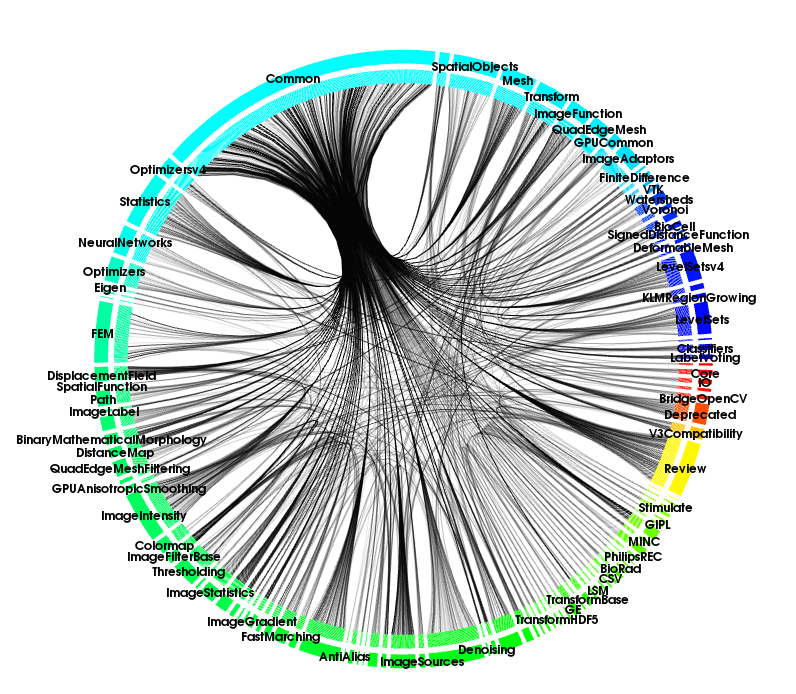
\includegraphics[width=0.4\textwidth]{itk_module_dependency.png}
    \caption{ An illustration on ITK modules' dependencies.}
    \label{fig:itk_module_dependency}
\end{figure}

\begin{figure}
  \centering
    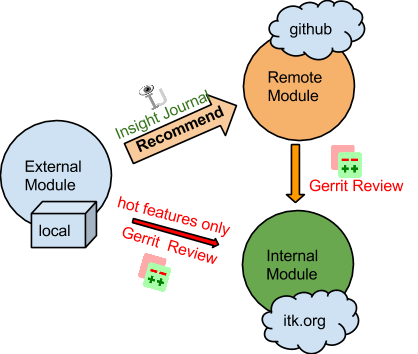
\includegraphics[width=0.3\textwidth]{itk_code_contribution.png}
    \caption{ Code contribution process in ITK.}
    \label{fig:itk_code_contribution}
\end{figure}


\begin{figure}
  \centering
    \includegraphics[width=1.0\textwidth]{itk_git_contributors.eps}
    \caption{Histogram of ITK contributors by number of commits in the repository since 2000.}
    \label{fig:ITKGitContributors}
\end{figure}


\begin{figure}
  \centering
    \includegraphics[width=0.5\textwidth]{gerrit_patch_set_histogram.eps}
    \caption{Histogram of the number of revisions (Patch Sets) for a given change.}
    \label{fig:gerrit_patch_set_histogram}
\end{figure}

\begin{figure}
  \centering
    \includegraphics[width=0.5\textwidth]{gerrit_fix_ups.eps}
    \caption{Fix-up commit percentage before and after peer code review.}
    \label{fig:gerrit_fix_ups}
\end{figure}

\begin{figure}
  \centering
    \showthe\textwidth
    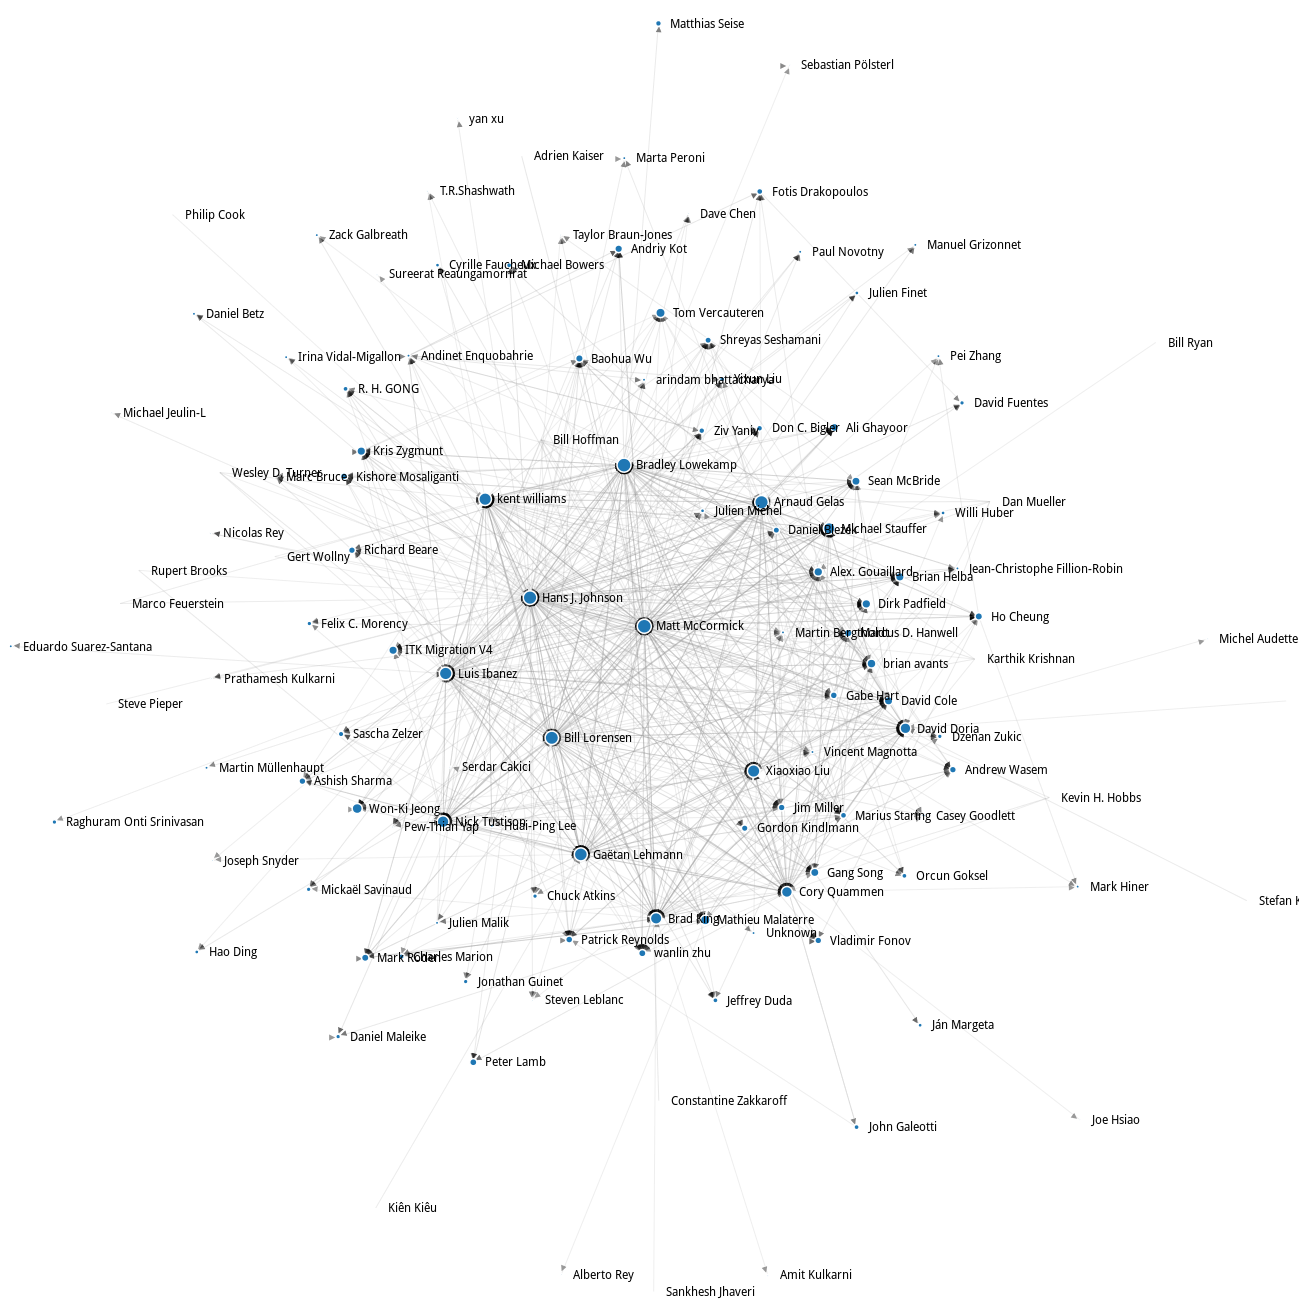
\includegraphics[width=1.0\textwidth]{GerritGraphRender.png}
    \caption{Peer code reviews graph.  Nodes are individual community members and
      size of the circle at the node is related logarithmically to the number of changes
      created by that community member.  The widths of the edges in this directed
      graph are logarithmically proportional to the number of reviews performed.}
    \label{fig:GerritGraph}
\end{figure}

\begin{figure}
  \centering
    \includegraphics[width=1.0\textwidth]{gerrit_closeness.eps}
    \caption{Normalized closeness centrality of peer code review graph versus
      the number of created changes.  Different connected components are shown
      in different colors.}
    \label{fig:GerritCloseness}
\end{figure}

\begin{figure}
  \centering
    \includegraphics[width=1.0\textwidth]{insight_journal_submissions.eps}
    \caption{Insight Journal submissions and reviews over the journal's
      likespan since 2005.}
    \label{fig:ij_submissions}
\end{figure}




\bibliography{frontiers}
\bibliographystyle{frontiersinSCNS&ENG} % for Science and Engineering articles


\end{document}
